\documentclass[sigplan,10pt,screen]{acmart}
\renewcommand\footnotetextcopyrightpermission[1]{}
\pagestyle{plain}

\usepackage{datetime}
\usepackage{url}
\usepackage{hyperref}
\usepackage{xspace}
\usepackage{amssymb}% http://ctan.org/pkg/amssymb
\usepackage{pifont}% http://ctan.org/pkg/pifont
\usepackage{todonotes}
\usepackage{cleveref}
\usepackage{tabularx}
\usepackage{booktabs}
\usepackage{multirow}
\usepackage{algorithm}
\usepackage[noend]{algpseudocode}
\usepackage{subcaption}

 \aboverulesep=0ex
 \belowrulesep=0ex
 
\crefformat{section}{\S#2#1#3}
\crefformat{subsection}{\S#2#1#3}
\crefformat{subsubsection}{\S#2#1#3}

\settopmatter{printacmref=false, printfolios=true, printccs=false}
\renewcommand\footnotetextcopyrightpermission[1]{}
\pagestyle{plain} 

\newcommand{\cmark}{\color{teal}\ding{51}}%
\newcommand{\xmark}{\color{red}\ding{55}}%

%\conferenceinfo{SOSP'17}{October 29--31, 2017, Shanghai, China}
%\copyrightyear{2017} 


% These only appear when the 'preprint' option is specified.
% Enabling these will cause the first page of the document to fail the 
% format check on HotCRP :-(
%\titlebanner{Under submission to SOSP 2017 - do not cite or distribute}
%\preprintfooter{Draft of {\currenttime}, \today{}}

% No date in title area.
\date{}

% Paper number and no. of pages as author
%\authorinfo{Paper \textbf{\#XX}}{NN pages}

\newcommand{\mycaption}[2]{\caption{\textbf{#1}. \textit{#2}}}
\newcommand{\sref}[1]{\S\ref{#1}}
\newcommand{\vheading}[1]{\vspace{0.05in}\noindent\textbf{#1}}
\newcommand{\viheading}[1]{\vspace{0.05in}\noindent\emph{#1}}
\newcommand{\vitem}[1]{\item\textbf{#1}}    
%\newcommand{\vb}[1]{\textbf{#1}}
\newcommand{\vb}[1]{\emph{#1}}
\newcommand{\fsync}{\texttt{fsync()}\xspace}
\newcommand{\etal}{\textit{et al.}\xspace}
\newcommand{\ie}{\textit{i.e.,}\xspace}
\newcommand{\eg}{\textit{e.g.,}\xspace}
\newcommand{\etc}{\textit{etc.}\xspace}
\newcommand*{\affmark}[1][*]{\textsuperscript{#1}}
\newcommand*{\affaddr}[1]{#1} % No op here. Customize it for different styles.


\usepackage{ifthen}
\newboolean{publicversion}
\setboolean{publicversion}{false}
\ifthenelse{\boolean{publicversion}}{
  \newcommand{\grumbler}[3]{}
}{
  \newcommand{\grumbler}[3]{\textcolor{#3}{\bf #1: #2}}
}

\newcommand{\vc}[1]{\grumbler{Vijay}{#1}{red}}
\newcommand{\DM}[1]{\grumbler{DM}{#1}{blue}}
\newcommand{\AT}[1]{\grumbler{AT}{#1}{orange}}

% Actual document begins below.
\begin{document}

\title{Model Checking Persistent Memory Data Structures}

\author{
  {\rm Soujanya Ponnapalli}
  \enspace 
  \vspace{8pt} \\
  \affaddr{Verification and Synthesis of Cyber Physical Systems (CS-395T or ASE-396)\\
  University of Texas at Austin}\hspace{10pt}
} %end author

\begin{abstract}
The advent of the Storage Class Memory (SCM) that is fast and byte-addressable
  similar to the Random Access Memory (DRAM or SRAM) and is persistent like the
  SSDs and hard disks, has attracted researchers to develop efficient data
  structures for adopting this persistent memory. However building efficient
  data structures for persistent memory that allow concurrent accesses to the
  data is challenging for two main reasons:
  1) The caches and registers remain volatile and require applications to flush
  the data from the caches to the persistent memory for durability.
  2) The cache flush instructions are reordered with load and store instructions
  in accordance to the memory model of the persistent memory and require
  applications to place fences to enforce ordering between these instructions.
  As fence and flush instructions incur heavy performance penalty and are
  crucial for correctness, the application developers should not insert fences
  unless they are strictly required for correctness. This tradeof complicates
  the design of persistent memory data structures and makes it extremely hard to
  reason about their correctness.

This paper aims at model checking persistent memory data structures for
  correctness and crash consistency by building a \emph{PM-Checker}. PM-Checker
  verifies that the data structure does not allow any instruction reorderings
  that can corrupt the data, and checks that crashing the data structure at any
  random point in time will not leave the persisted data in an inconsistent
  state. Overall, this paper models the persistent memory, formulizes the
  specifications for correctness and crash consistency and verifies
  state-of-the-art persistent memory data structures.
\end{abstract}


\maketitle

\section{Problem Definition}

\section{PM-CHECKER}

\begin{figure}[t]
    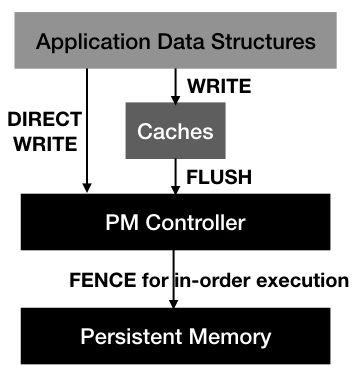
\includegraphics[width=\columnwidth]{figures/nvm-architecture.jpg}
    \caption{\emph{The architecture of Persitent Memory.}}
    \label{fig:architecture}
    \vspace{-0.3in}
\end{figure}


PM-CHECKER\footnote{https://github.com/SoujanyaPonnapalli/ASE-396-CourseProject}
models the architecture as shown in the Figure-\cite{fig-nvm-architecture}.

\section{Desired Outcomes}

\section{Milestones}

\section{Conclusion}


\clearpage

\bibliographystyle{ACM-Reference-Format}
\bibliography{ref}

\end{document}
